%
% Barren Planet - User Manual
% Main document source
%
% Copyright (C) Damian Gareth Walker 2022
% Manual Sections: Playing With Friends
%
% Structure:
% Hotseat Play
% Play-by-mail
%

% Chapter Title
\chapter{Playing With Better Opponents}

% Introductory
\noindent
So far you have played against the computer on its easiest setting. If you want the computer to be more of a challenge, there are harder computer opponents available. As well as {\it Computer (Easy)}, there are player settings for {\it Computer (Fair)} and {\it Computer (Hard)}. These are all available on the {\it Set up Game} screen.

Beating up a computer opponent can be fun, but the most satisfying victories are those against human opponents. So once you have won a game or two against the computer, it's time to invite a friend to play. There are two ways to do this: Hotseat Play and Play-by-Mail.

% Hotseat Play
\section{Hotseat Play}

% What is Hotseat Play
\noindent
Hotseat Play is where two people take turns at the same computer, one vacating the seat when it's the other person's turn to play. It is the simplest kind of two-player game to set up.

% Setting up the Game
On the {\it New Game} screen, make sure {\it Game:} is set to {\it New Game}. Then set both Nuvutech and Avuscorp to {\it Human}. Then you can tap {\it fire} to choose the {\it Start game} menu option. It is up to the players to agree who is playing which side.

% The Security Screen
Instead of going straight to the {\it Mission Briefing} screen, you will be presented first with what's termed the {\it Security Screen}. This shows the emblem of the player whose turn it is. The other player should find something to look at other than the screen, and the player whose turn it is can tap {\it fire} to choose the {\it Proceed} option. After this, the Mission Briefing and other play screens appear as normal.

% The Security screen image
\begin{figure}[h]
  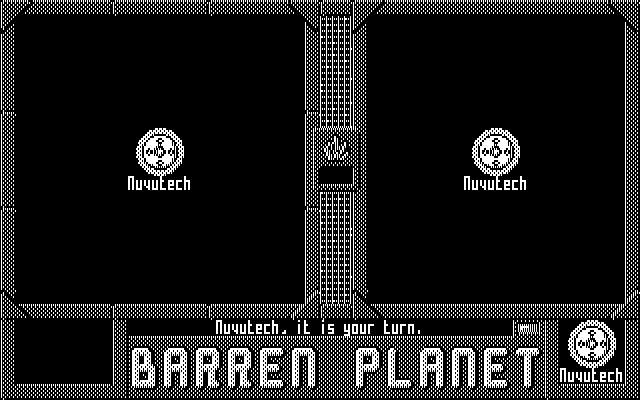
\includegraphics[width=\textwidth]{security}
  \caption{The ``Security'' screen}
\end{figure}

% Not Real Security
Although called the {\it Security Screen}, this initial screen offers no real security. Its real purpose is to let players know whose turn it is, and to prevent one player accidentally trying to play when it is not their turn. It appears every time control passes from one player to the other.

% Play-by-Mail
\section{Play-by-Mail}

% Introduction
\noindent
Sometimes it's not practical for two players to get together in the same place at the same time. For those occasions, {\bf \it Barren Planet} offers a {\it Play-by-Mail} feature. This allows each player to sit at their own computer and take their turn at a time that's convenient. After each player has taken their turn, a {\it Turn File} is generated that can be delivered to their opponent for them to take their turn.

% Setting Up
First the players need to agree who is playing which side, and who will set the game up. For the purpose of this description, let's assume that you are setting up the game. From the {\it New Game} screen, set {\it Game:} to {\it New Game}, mark your own side as {\it Human}, and your opponent's side as {\it PBM}. Then tap {\it fire} to choose {\it Start Game} from the menu.

% Setting up a new PBM game image
\begin{figure}[h]
  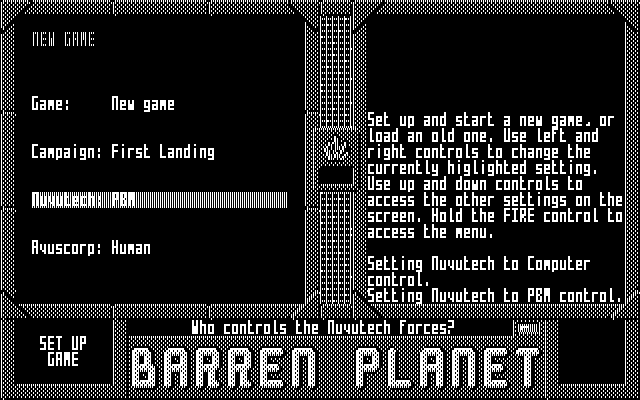
\includegraphics[width=\textwidth]{new-pbm}
  \caption{Setting up a new PBM game}
\end{figure}

% First Turn
If you are randomly allotted the first turn, then you will get to play it as normal, going through the Mission Briefing and Player Turn screens. Once you have ended your turn, or if the game has decided your opponent takes the first turn, control will pass to the {\it Remote Player} screen. The Turn File will be generated, and a message will tell you its file name.

% The PBM Turn send screen image
\begin{figure}[h]
  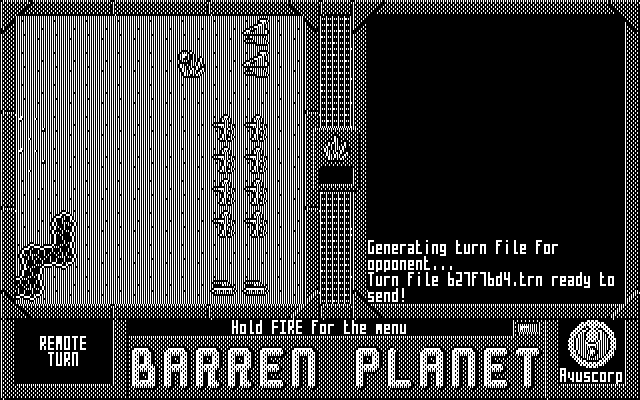
\includegraphics[width=\textwidth]{turn-send}
  \caption{The turn is ready to send to the Nuvutech player}
\end{figure}

% Sending the Turn File
It's then up to you to get the turn file to your opponent with whatever means necessary. You can copy it to a floppy disk and post it to your opponent, or hand deliver it if your opponent is someone you meet regularly. Or you can send it as an attachment using electronic mail.

% The PBM Turn receive screen image
\begin{figure}[h]
  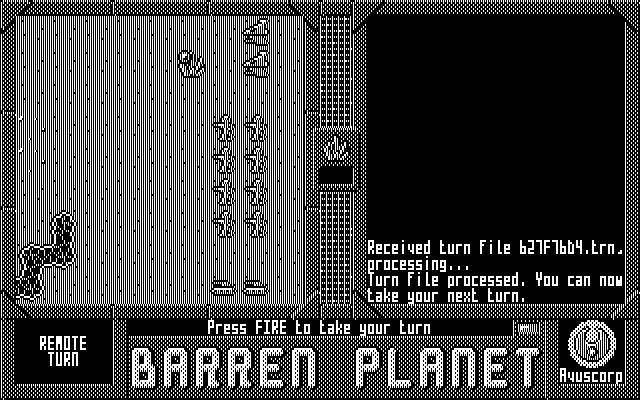
\includegraphics[width=\textwidth]{turn-receive}
  \caption{The turn has been received from the Avuscorp player}
\end{figure}

% Receiving the First Turn File
If you're the recipient of the Turn File, you must copy it to your {\bf \it Barren Planet} disk or directory before starting the program. A brief message on the {\it New Game} screen will confirm that the turn file has been read, and which game it applies to. The turn file will then be deleted. You can then start the game and take your turn. Once you end your turn, the program will generate another turn file for you to return to your opponent.
